\chapter{Mod\`eles de Machine Learning}
\label{ch:modeles}

\section{R\'egression lin\'eaire}
\label{sec:regression_lineaire}

\index{r\'egression lin\'eaire}

\begin{definition}[R\'egression lin\'eaire]
La \textbf{r\'egression lin\'eaire} mod\'elise la relation entre une variable cible $y$ et des variables explicatives $\mathbf{x}$~:
\[
y = \mathbf{X}\boldsymbol{\beta} + \varepsilon
\]
o\`u $\boldsymbol{\beta}$ est le vecteur des coefficients et $\varepsilon$ est le terme d'erreur.
\end{definition}

\begin{theoreme}[Moindres carr\'es ordinaires (MCO)]
\index{moindres carr\'es ordinaires}\index{MCO}
L'estimateur MCO minimise la somme des carr\'es des r\'esidus~:
\[
\hat{\boldsymbol{\beta}} = \arg\min_{\boldsymbol{\beta}} \| \mathbf{y} - \mathbf{X}\boldsymbol{\beta} \|^2 = (\mathbf{X}^\top \mathbf{X})^{-1}\mathbf{X}^\top \mathbf{y}
\]
\end{theoreme}

\begin{definition}[Coefficient de d\'etermination $R^2$]
\index{coefficient de d\'etermination}\index{R carre@$R^2$}
Le $R^2$ mesure la proportion de la variance expliqu\'ee par le mod\`ele~:
\[
R^2 = 1 - \frac{\sum_{i=1}^{n}(y_i - \hat{y}_i)^2}{\sum_{i=1}^{n}(y_i - \bar{y})^2} \in (-\infty, 1]
\]
Un $R^2$ proche de 1 indique un bon ajustement.
\end{definition}

\begin{codeblock}[title=\textbf{Python}]
\begin{minted}{python}
import seaborn as sns
import pandas as pd
from sklearn.linear_model import LinearRegression
from sklearn.model_selection import train_test_split
from sklearn.metrics import mean_squared_error, r2_score

# Chargement du jeu de donn\'ees tips
tips = sns.load_dataset('tips')
X = tips[['total_bill', 'size']]
y = tips['tip']

X_train, X_test, y_train, y_test = train_test_split(
    X, y, test_size=0.3, random_state=42
)

# R\'egression lin\'eaire
reg = LinearRegression()
reg.fit(X_train, y_train)
y_pred = reg.predict(X_test)

print(f"Coefficients : {reg.coef_}")
print(f"Intercept    : {reg.intercept_:.4f}")
print(f"R\u00b2 (test)    : {r2_score(y_test, y_pred):.4f}")
print(f"RMSE (test)  : {mean_squared_error(y_test, y_pred, squared=False):.4f}")
\end{minted}
\end{codeblock}

\begin{codeoutput}
\begin{minted}{text}
Coefficients : [0.0932 0.1803]
Intercept    : 0.6689
R² (test)    : 0.4616
RMSE (test)  : 1.0459
\end{minted}
\end{codeoutput}

\section{R\'egression logistique}
\label{sec:regression_logistique}

\index{r\'egression logistique}\index{sigmo\"ide}

\begin{definition}[R\'egression logistique]
La \textbf{r\'egression logistique} est un mod\`ele de \textbf{classification binaire}\index{classification binaire}. Elle mod\'elise la probabilit\'e d'appartenance \`a la classe 1 via la fonction sigmo\"ide~:
\[
P(y=1 \mid \mathbf{x}) = \sigma(\mathbf{x}^\top \boldsymbol{\beta}) = \frac{1}{1 + e^{-\mathbf{x}^\top \boldsymbol{\beta}}}
\]
\end{definition}

\begin{center}
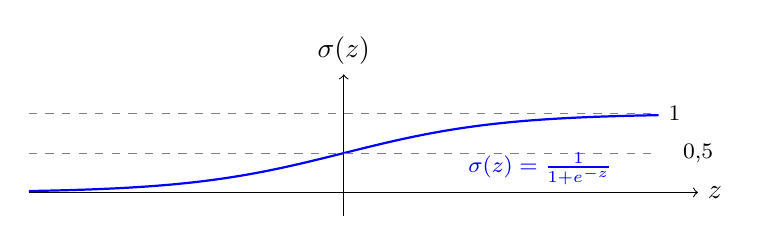
\begin{tikzpicture}
    \draw[->] (-4,0) -- (4.5,0) node[right] {$z$};
    \draw[->] (0,-0.3) -- (0,1.5) node[above] {$\sigma(z)$};
    \draw[blue, thick, domain=-4:4, smooth, samples=100] plot (\x, {1/(1+exp(-\x))});
    \draw[dashed, gray] (-4,1) -- (4,1);
    \draw[dashed, gray] (-4,0.5) -- (4,0.5);
    \node[font=\footnotesize] at (4.2, 1) {$1$};
    \node[font=\footnotesize] at (4.5, 0.5) {$0{,}5$};
    \node[font=\footnotesize, blue] at (2.5, 0.3) {$\sigma(z) = \frac{1}{1+e^{-z}}$};
\end{tikzpicture}
\end{center}

\begin{codeblock}[title=\textbf{Python}]
\begin{minted}{python}
from sklearn.linear_model import LogisticRegression
from sklearn.preprocessing import LabelEncoder

# Titanic : classification binaire (survie)
titanic = sns.load_dataset('titanic').dropna(subset=['age', 'fare'])
X_ti = titanic[['age', 'fare', 'pclass']]
y_ti = titanic['survived']

X_train, X_test, y_train, y_test = train_test_split(
    X_ti, y_ti, test_size=0.3, random_state=42
)

logreg = LogisticRegression(max_iter=1000)
logreg.fit(X_train, y_train)
print(f"Exactitude (train) : {logreg.score(X_train, y_train):.4f}")
print(f"Exactitude (test)  : {logreg.score(X_test, y_test):.4f}")
\end{minted}
\end{codeblock}

\begin{codeoutput}
\begin{minted}{text}
Exactitude (train) : 0.6962
Exactitude (test)  : 0.6878
\end{minted}
\end{codeoutput}

\section{Arbres de d\'ecision}
\label{sec:arbres_decision}

\index{arbre de d\'ecision}\index{DecisionTreeClassifier}

\begin{definition}[Arbre de d\'ecision]
Un \textbf{arbre de d\'ecision} partitionne l'espace des variables explicatives par des tests binaires successifs, formant une structure arborescente. Chaque feuille correspond \`a une pr\'ediction.
\end{definition}

\begin{center}
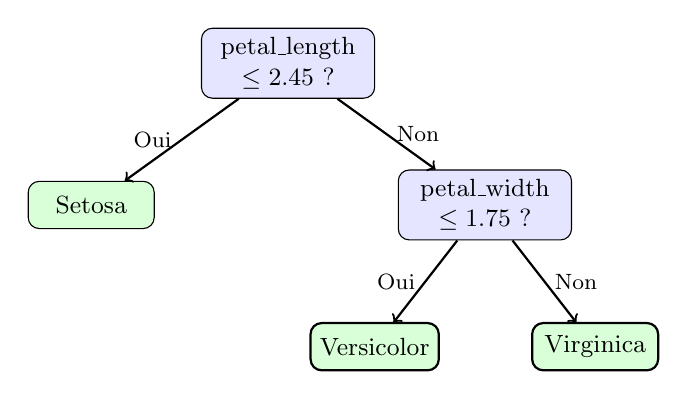
\begin{tikzpicture}[
    node/.style={rectangle, draw, rounded corners, fill=blue!10, minimum width=2.2cm, minimum height=0.7cm, align=center, font=\small},
    leaf/.style={rectangle, draw, rounded corners, fill=green!15, minimum width=1.6cm, minimum height=0.6cm, align=center, font=\small},
    edge from parent/.style={draw, ->, thick},
    level 1/.style={sibling distance=5cm, level distance=1.8cm},
    level 2/.style={sibling distance=2.8cm, level distance=1.8cm}
]
\node[align=center,node] {petal\_length\\$\leq 2.45$~?}
    child {
        node[leaf] {Setosa}
        edge from parent node[left, font=\footnotesize] {Oui}
    }
    child {
        node[node] {petal\_width\\$\leq 1.75$~?}
        child {
            node[leaf] {Versicolor}
            edge from parent node[left, font=\footnotesize] {Oui}
        }
        child {
            node[leaf] {Virginica}
            edge from parent node[right, font=\footnotesize] {Non}
        }
        edge from parent node[right, font=\footnotesize] {Non}
    };
\end{tikzpicture}
\end{center}

\begin{codeblock}[title=\textbf{Python}]
\begin{minted}{python}
from sklearn.tree import DecisionTreeClassifier
from sklearn.datasets import load_iris
from sklearn.model_selection import cross_val_score

iris = load_iris()
X, y = iris.data, iris.target

# Arbre avec profondeur maximale limit\'ee
tree = DecisionTreeClassifier(max_depth=3, random_state=42)
scores = cross_val_score(tree, X, y, cv=5)
print(f"Arbre (max_depth=3) : {scores.mean():.4f} (+/- {scores.std():.4f})")

# Arbre sans limite de profondeur
tree_full = DecisionTreeClassifier(random_state=42)
scores_full = cross_val_score(tree_full, X, y, cv=5)
print(f"Arbre (sans limite) : {scores_full.mean():.4f} (+/- {scores_full.std():.4f})")
\end{minted}
\end{codeblock}

\begin{codeoutput}
\begin{minted}{text}
Arbre (max_depth=3) : 0.9667 (+/- 0.0211)
Arbre (sans limite) : 0.9533 (+/- 0.0327)
\end{minted}
\end{codeoutput}

\begin{attention}
Un arbre sans limite de profondeur (\py{max_depth=None}) risque de \textbf{sur-apprendre}. Limitez la profondeur ou le nombre minimum d'\'echantillons par feuille (\py{min_samples_leaf}).
\end{attention}

\section{For\^ets al\'eatoires}
\label{sec:forets_aleatoires}

\index{for\^et al\'eatoire}\index{RandomForestClassifier}\index{bagging}\index{ensemble}

\begin{definition}[For\^et al\'eatoire]
Une \textbf{for\^et al\'eatoire} (\textit{Random Forest}) est un \textbf{ensemble} de $B$ arbres de d\'ecision entra\^in\'es sur des sous-\'echantillons al\'eatoires des donn\'ees (\textit{bagging}). La pr\'ediction finale est le \textbf{vote majoritaire} (classification) ou la \textbf{moyenne} (r\'egression).
\end{definition}

\begin{codeblock}[title=\textbf{Python}]
\begin{minted}{python}
from sklearn.ensemble import RandomForestClassifier

rf = RandomForestClassifier(n_estimators=100, max_depth=5, random_state=42)
scores_rf = cross_val_score(rf, X, y, cv=5)
print(f"For\^et al\'eatoire : {scores_rf.mean():.4f} (+/- {scores_rf.std():.4f})")
\end{minted}
\end{codeblock}

\begin{codeoutput}
\begin{minted}{text}
For\^et al\'eatoire : 0.9667 (+/- 0.0211)
\end{minted}
\end{codeoutput}

\section{K plus proches voisins (KNN)}
\label{sec:knn_detail}

\index{KNN}\index{distance euclidienne}

\begin{definition}[KNN]
Le classifieur \textbf{$k$ plus proches voisins} attribue \`a une nouvelle observation la classe majoritaire parmi ses $k$ voisins les plus proches selon une m\'etrique de distance (g\'en\'eralement euclidienne)~:
\[
d(\mathbf{x}, \mathbf{x}') = \sqrt{\sum_{j=1}^{p}(x_j - x'_j)^2}
\]
\end{definition}

\begin{bonnepratique}
La performance de KNN d\'epend fortement de l'\textbf{\'echelle} des variables. Normalisez toujours vos donn\'ees avant d'utiliser KNN~:
\begin{minted}{python}
from sklearn.preprocessing import StandardScaler
scaler = StandardScaler()
X_scaled = scaler.fit_transform(X)
\end{minted}
\end{bonnepratique}

\section{K-Means~: clustering}
\label{sec:kmeans}

\index{K-Means}\index{clustering}\index{m\'ethode du coude}

\begin{definition}[K-Means]
\textbf{K-Means} est un algorithme d'apprentissage \textbf{non supervis\'e} qui partitionne $n$ observations en $K$ groupes (\textit{clusters}) en minimisant l'inertie~:
\[
\mathcal{J} = \sum_{k=1}^{K}\sum_{\mathbf{x}_i \in C_k} \| \mathbf{x}_i - \boldsymbol{\mu}_k \|^2
\]
o\`u $\boldsymbol{\mu}_k$ est le centro\"ide du cluster $C_k$.
\end{definition}

\begin{center}
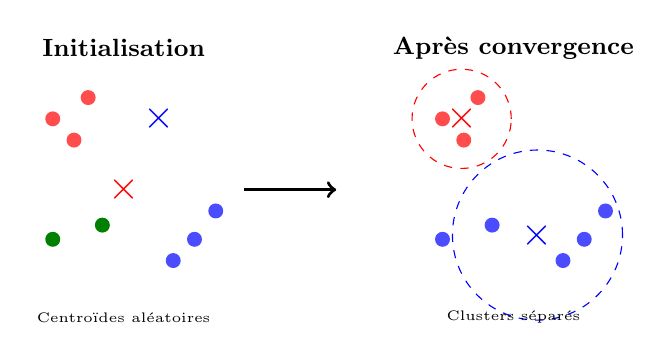
\begin{tikzpicture}[scale=0.9]
    % It\'eration 1
    \begin{scope}[shift={(-4,0)}]
        \node[font=\bfseries\small] at (1.5, 3.5) {Initialisation};
        \fill[red!70] (0.5, 2.5) circle (3pt);
        \fill[red!70] (1.0, 2.8) circle (3pt);
        \fill[red!70] (0.8, 2.2) circle (3pt);
        \fill[blue!70] (2.5, 0.8) circle (3pt);
        \fill[blue!70] (2.8, 1.2) circle (3pt);
        \fill[blue!70] (2.2, 0.5) circle (3pt);
        \fill[green!50!black] (1.2, 1.0) circle (3pt);
        \fill[green!50!black] (0.5, 0.8) circle (3pt);
        \node[red, font=\Large] at (1.5, 1.5) {$\times$};
        \node[blue, font=\Large] at (2.0, 2.5) {$\times$};
        \node[font=\tiny] at (1.5, -0.3) {Centro\"ides al\'eatoires};
    \end{scope}
    % Fl\`eche
    \draw[->, very thick] (-0.8, 1.5) -- (0.5, 1.5);
    % It\'eration 2
    \begin{scope}[shift={(1.5,0)}]
        \node[font=\bfseries\small] at (1.5, 3.5) {Apr\`es convergence};
        \fill[red!70] (0.5, 2.5) circle (3pt);
        \fill[red!70] (1.0, 2.8) circle (3pt);
        \fill[red!70] (0.8, 2.2) circle (3pt);
        \fill[blue!70] (2.5, 0.8) circle (3pt);
        \fill[blue!70] (2.8, 1.2) circle (3pt);
        \fill[blue!70] (2.2, 0.5) circle (3pt);
        \fill[blue!70] (1.2, 1.0) circle (3pt);
        \fill[blue!70] (0.5, 0.8) circle (3pt);
        \node[red, font=\Large] at (0.77, 2.5) {$\times$};
        \node[blue, font=\Large] at (1.84, 0.86) {$\times$};
        \draw[red, dashed] (0.77, 2.5) circle (0.7cm);
        \draw[blue, dashed] (1.84, 0.86) circle (1.2cm);
        \node[font=\tiny] at (1.5, -0.3) {Clusters s\'epar\'es};
    \end{scope}
\end{tikzpicture}
\end{center}

\begin{codeblock}[title=\textbf{Python}]
\begin{minted}{python}
from sklearn.cluster import KMeans
from sklearn.datasets import load_iris
import numpy as np

iris = load_iris()
X = iris.data

# M\'ethode du coude
inertias = []
K_range = range(1, 11)
for k in K_range:
    km = KMeans(n_clusters=k, n_init=10, random_state=42)
    km.fit(X)
    inertias.append(km.inertia_)

print("K  | Inertie")
print("-" * 20)
for k, inertia in zip(K_range, inertias):
    print(f"{k:2d} | {inertia:.1f}")
\end{minted}
\end{codeblock}

\begin{codeoutput}
\begin{minted}{text}
K  | Inertie
--------------------
 1 | 681.4
 2 | 152.3
 3 | 78.9
 4 | 57.3
 5 | 46.5
 6 | 39.0
 7 | 34.2
 8 | 29.9
 9 | 27.8
10 | 25.4
\end{minted}
\end{codeoutput}

\begin{intuition}
La \textbf{m\'ethode du coude}\index{m\'ethode du coude} consiste \`a chercher le point o\`u l'inertie cesse de diminuer significativement. Ici, $K=3$ correspond au <<~coude ~>>, coh\'erent avec les 3 esp\`eces d'Iris.
\end{intuition}

\section{Tableau comparatif des mod\`eles}

\begin{center}
\begin{tabular}{llccc}
\toprule
\textbf{Mod\`ele} & \textbf{Type} & \textbf{Interpr\'etable} & \textbf{Normalisation} & \textbf{Hyperparam\`etres cl\'es} \\
\midrule
R\'eg.\ lin\'eaire & R\'egression & Oui & Non & --- \\
R\'eg.\ logistique & Classification & Oui & Oui & \py{C} \\
Arbre de d\'ecision & Les deux & Oui & Non & \py{max_depth} \\
For\^et al\'eatoire & Les deux & Non & Non & \py{n_estimators}, \py{max_depth} \\
KNN & Les deux & Non & Oui & \py{n_neighbors} \\
K-Means & Clustering & Moyen & Oui & \py{n_clusters} \\
\bottomrule
\end{tabular}
\end{center}

\section{Exercices}

\begin{exercice}[$\star$]
Chargez le jeu de donn\'ees \texttt{tips} de seaborn. Entra\^inez une r\'egression lin\'eaire pour pr\'edire le pourboire (\py{tip}) \`a partir de \py{total_bill} uniquement. Affichez le coefficient, l'intercept et le $R^2$.
\end{exercice}

\begin{exercice}[$\star$]
Sur le jeu Iris, comparez l'exactitude (validation crois\'ee \`a 5 plis) d'un arbre de d\'ecision (\py{max_depth=3}), d'une for\^et al\'eatoire (100 arbres) et de KNN ($k=5$).
\end{exercice}

\begin{exercice}[$\star\star$]
Chargez le jeu \texttt{titanic} de seaborn. Pr\'eparez les donn\'ees (supprimez les lignes avec valeurs manquantes dans \py{age}, \py{fare}~; utilisez \py{pclass}, \py{age}, \py{fare}, \py{sex} encod\'e). Comparez la r\'egression logistique et une for\^et al\'eatoire pour pr\'edire \py{survived}.
\end{exercice}

\begin{exercice}[$\star\star$]
Appliquez K-Means avec $K=3$ sur les donn\'ees Iris (sans les \'etiquettes). Comparez les clusters obtenus avec les vraies esp\`eces \`a l'aide d'un tableau crois\'e (\py{pd.crosstab}).
\end{exercice}

\begin{exercice}[$\star\star\star$]
Chargez le jeu \py{fetch_california_housing()} de scikit-learn. Entra\^inez une r\'egression lin\'eaire et une for\^et al\'eatoire. Comparez les $R^2$ et RMSE sur l'ensemble de test. Tracez les pr\'edictions vs.\ les valeurs r\'eelles pour les deux mod\`eles.
\end{exercice}

\begin{exercice}[$\star\star\star$]
Impl\'ementez l'algorithme KNN <<~\`a la main ~>> (sans scikit-learn) en utilisant NumPy. Testez-le sur Iris et comparez vos r\'esultats avec \py{KNeighborsClassifier}.
\end{exercice}

\begin{formules}
\textbf{R\'esum\'e du chapitre~\ref{ch:modeles}}
\begin{itemize}
    \item \textbf{R\'egression lin\'eaire}~: $y = \mathbf{X}\boldsymbol{\beta} + \varepsilon$, MCO~: $\hat{\boldsymbol{\beta}} = (\mathbf{X}^\top\mathbf{X})^{-1}\mathbf{X}^\top\mathbf{y}$.
    \item \textbf{R\'egression logistique}~: $P(y{=}1|\mathbf{x}) = \sigma(\mathbf{x}^\top\boldsymbol{\beta})$, classification binaire.
    \item \textbf{Arbre de d\'ecision}~: partitions successives, contr\^oler \py{max_depth}.
    \item \textbf{For\^et al\'eatoire}~: ensemble d'arbres par \textit{bagging}, plus robuste.
    \item \textbf{KNN}~: vote des $k$ plus proches voisins, n\'ecessite normalisation.
    \item \textbf{K-Means}~: clustering non supervis\'e, minimise l'inertie $\mathcal{J}$.
    \item \textbf{M\'ethode du coude}~: choisir $K$ au point d'inflexion de l'inertie.
\end{itemize}
\end{formules}
